% ---------------------------------------------------------------------------- %
\chapter{Experimental Setup}
\label{ch:experimentalSetup}
% ---------------------------------------------------------------------------- %

\begin{itemize}\tightlist
    \item
        How does the device itself look, physically?
    \item
        What considerations must  be taken when trying to put  the device into
        operation?
    \item
        How does the resulting setup look, w/ all devices and their settings?
    \item
        How were the measurements conducted (methodology)?
    \item
        How were the results obtained and evaluated?
\end{itemize}

%\todo[inline]{Fundamental experimental setup w/ Raspbi, test board, PC}
%\missingfigure{Block Diagram: Raspbi, Test Board, PC}

\fref{fig:experimentDiagram} shows  a schematic  overview of  the experimental
setup as  used in the tests  documented in this report. Note  that the \raspi~
requires  both the  \signal{clk} and  \signal{vss} from  the test  board as  a
reference  in addition  to the  bit stream  itself. A PC  is connected  to the
\raspi~ for convenience via SSH, though this is not strictly necessary.

\begin{figure}
    \sisetup{range-phrase = { \ldots }}
\sisetup{list-pair-separator = {/}}
\begin{tikzpicture}[%
        align=center,
        %text=solarized-base02,
        %draw=solarized-base02,
        %remember picture,
        %overlay,
    ]
    \small
    \sffamily
    %\begin{scope}[x={(0mm,0.95\textwidth)},y={(0mm,50mm)}]

    %\draw [help lines] (0,0) grid (10,-15);

    \begin{scope}[
        x={(0mm,135mm)},
        every node/.style = {
            %double,
            draw,
            inner sep = 2mm,
            rounded corners = 1mm
        },
        sign/.style={
            inner sep=2mm,
            rounded corners=1mm,
            fill=solarized-magenta,
            text=solarized-base3,
        },
        testboard/.style={
            fill=solarized-magenta,
            draw=solarized-base03,
            text=solarized-base3,
        },
        raspi/.style={
            fill=solarized-cyan,
            draw=solarized-base03,
            text=solarized-base3,
        },
        pc/.style={
            fill=solarized-cyan,
            draw=solarized-base03,
            text=solarized-base3,
        },
        3v/.style={
            signal,
            signal to = east,
            fill=solarized-blue,
            draw=solarized-base03,
            text=solarized-base3,
        },
        1.5v/.style={
            signal,
            signal to = east,
            fill=green!55!black,
            draw=solarized-base03,
            text=solarized-base3,
        },
        ibias/.style={
            signal,
            signal to = east,
            fill=red!95!black,
            draw=solarized-base03,
            text=solarized-base3,
        },
        clk/.style={
            signal,
            signal to = west,
            fill=green!75!black,
            draw=solarized-base03,
            text=solarized-base03,
        },
        gnd/.style={
            signal,
            signal to = east,
            fill=black,
            draw=black,
            text=solarized-base3,
        },
        vin/.style={
            signal,
            signal to = east,
            fill=solarized-red,
            draw=solarized-base03,
            text=solarized-base3,
        },
        bitStream/.style={
            signal,
            signal to = east,
            fill=yellow!90!black,
            draw=solarized-base03,
            text=solarized-base03,
        }
    ]

        \node (3v)    [anchor=west,3v]    at (0,0)     {\texttt{VDDD}, \texttt{VDDA}: \SI{3}{\volt}};
        \node (15v)   [anchor=west,1.5v]  at (0,-8mm)  {\texttt{VGNDA}: \SI{1.5}{\volt}};
        \node (vin)   [anchor=west,vin]   at (0,-16mm) {\texttt{vin}: \SIrange{0.5}{2.5}{\volt}};
        \node (ibias) [anchor=west,ibias] at (0,-24mm) {\texttt{ibias}: \SI{120}{\micro\ampere}};
        \node (gnd)   [anchor=west,gnd]   at (0,-32mm) {\texttt{VSS}: \SI{0}{\volt}};
        \node (gnd2)  [anchor=west,gnd]   at (74mm,-32mm) {\texttt{VSS}: \SI{0}{\volt}};

        \node (testBoard) [minimum height=40mm,minimum width=19mm,right=17 mm of vin,testboard] {\rotatebox{90}{Test Board}};


        \node (clk) [anchor=west,clk] at (101mm,0) {\texttt{clk}: \SIlist{0;3}{\volt}};
        \node (bitStream) [anchor=west,bitStream] at (74mm,-16mm) {\texttt{bit\_stream}};

        \node (raspi) [raspi] at (115mm,-16mm) {Raspberyy Pi};
        \node (pc) [pc] at (135mm,-16mm) {PC};
    \end{scope}


    \begin{scope}[
        %every node/.style={ },
            rounded corners,
            every path/.append style={draw=solarized-base03,},
    ]
        %\draw[-latex] (3v) -- (53mm,0);
        \draw[-latex] (3v)    to[out=0,in=180] (53mm,0);
        \draw[-latex] (15v)   to[out=0,in=180] (53mm,-8mm);
        \draw[-latex] (vin)   to[out=0,in=180] (53mm,-16mm);
        \draw[-latex] (ibias) to[out=0,in=180] (53mm,-24mm);
        \draw[-latex] (gnd)   to[out=0,in=180] (53mm,-32mm);

        \draw[-latex] (testBoard) -- (bitStream);
        \draw[-latex] (bitStream) -- (raspi);
        \draw[latex-latex] (raspi) -- (pc);

        \draw[-latex] (clk) -- (71.5mm,0);
        \draw[-latex] (clk) -- (raspi);
        \draw[-latex] (71.5mm,-32mm) -- (gnd2);
        \draw[-latex] (gnd2) -| (raspi);

        %\draw[line width=2pt,-latex] (oosk1) --  node[midway, anchor = west] {DC-Leitung} (oosk2);
    \end{scope}

\end{tikzpicture}

    \caption{%
        Experimental    setup   with    signal    and   supply    connections.
        \emph{Note}: Signal colors roughly correspond to wire colors used.%
    }
    \label{fig:experimentDiagram}
\end{figure}


% ---------------------------------------------------------------------------- %
\section{Putting the Sensor IC Into Operation}
\label{sec:ICintoOperation}
% ---------------------------------------------------------------------------- %

This  section  will  detail  the  steps  needed to  put  the  Sensor  IC  into
operation. Some  of  this  information  will be  redundant  with  the  reports
\cite{ref:burgherr},  \cite{ref:gloor} and  \cite{ref:baier},  but  we aim  to
provide a  convenient guide to  this process in  a single place,  thus sparing
future teams the effort of needing  to assemble this information from multiple
sources, which is both a time-consuming and error-prone process.
\todo[noline]{Make direct references to pages/tables in other reports?}
\todo[noline]{handling with care and all that stuff}

Fundamentally, putting the chip into operation consists of the following steps:
\begin{itemize}\tightlist
    \item
        Determine bias resistor setting.
    \item
        Set DIP switches to the appropriate values.
    \item
        Connect supply voltages and bias current supply.
    \item
        Set up \raspi.
    \item
        Connect \raspi~and test board.
\end{itemize}

These  steps  will   be  outlined  in  the  following   sections,  along  with
supplementary information where appropriate. Before delving into the operation
of the test board, a brief outline of its elements and functions will be given
in the next section.

% ---------------------------------------------------------------------------- %
\subsection{Basic Layout of PCB}
\label{subsec:PCBLayout}
% ---------------------------------------------------------------------------- %

A test board, depicted in figure \fref{fig:pcbOverview}, has been developed in
\todo{Insert Reference to p.1-32 in Burgherr} to enable convenient examination
of the sensor IC.  Seven industrial plugs are located on the board's left-hand
side \todo{correct name?}. They  can be used for the  various supply voltages,
signal input as well as bias current input and ground.

\todo[noline]{How to operate chip socket}

\begin{figure}
    \centering
    %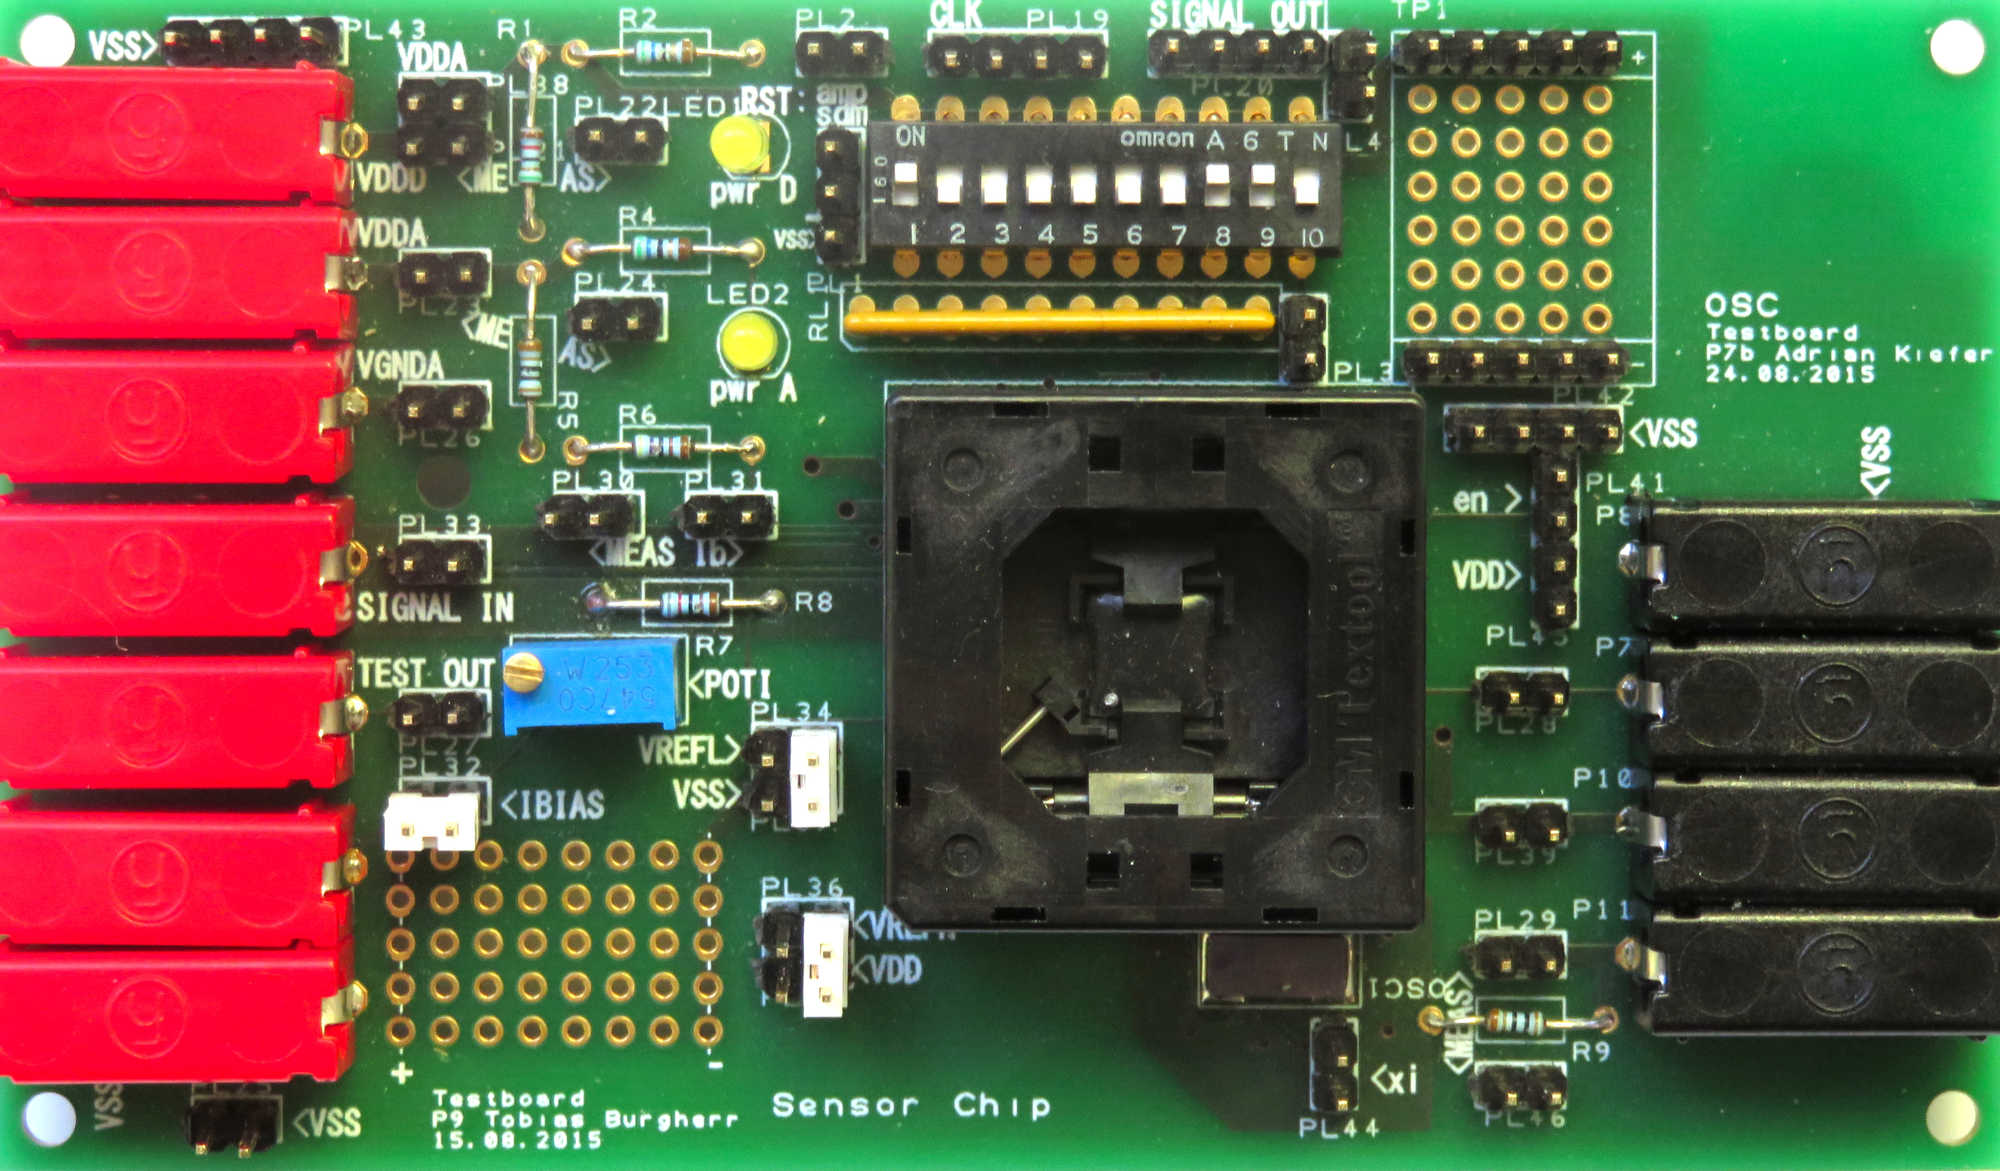
\includegraphics[width=\textwidth]{images/pcb/pcbOverview.jpeg}
    \newcommand{\plugtext}[1]{\textbf{\texttt{\Large{#1}}}}

\begin{tikzpicture}
    \begin{scope}[x={(0mm,135mm)},y={(0mm,79mm)},line width=1pt,cap=round]
        \node[anchor=south west,inner sep=0mm] at (0mm,0mm) {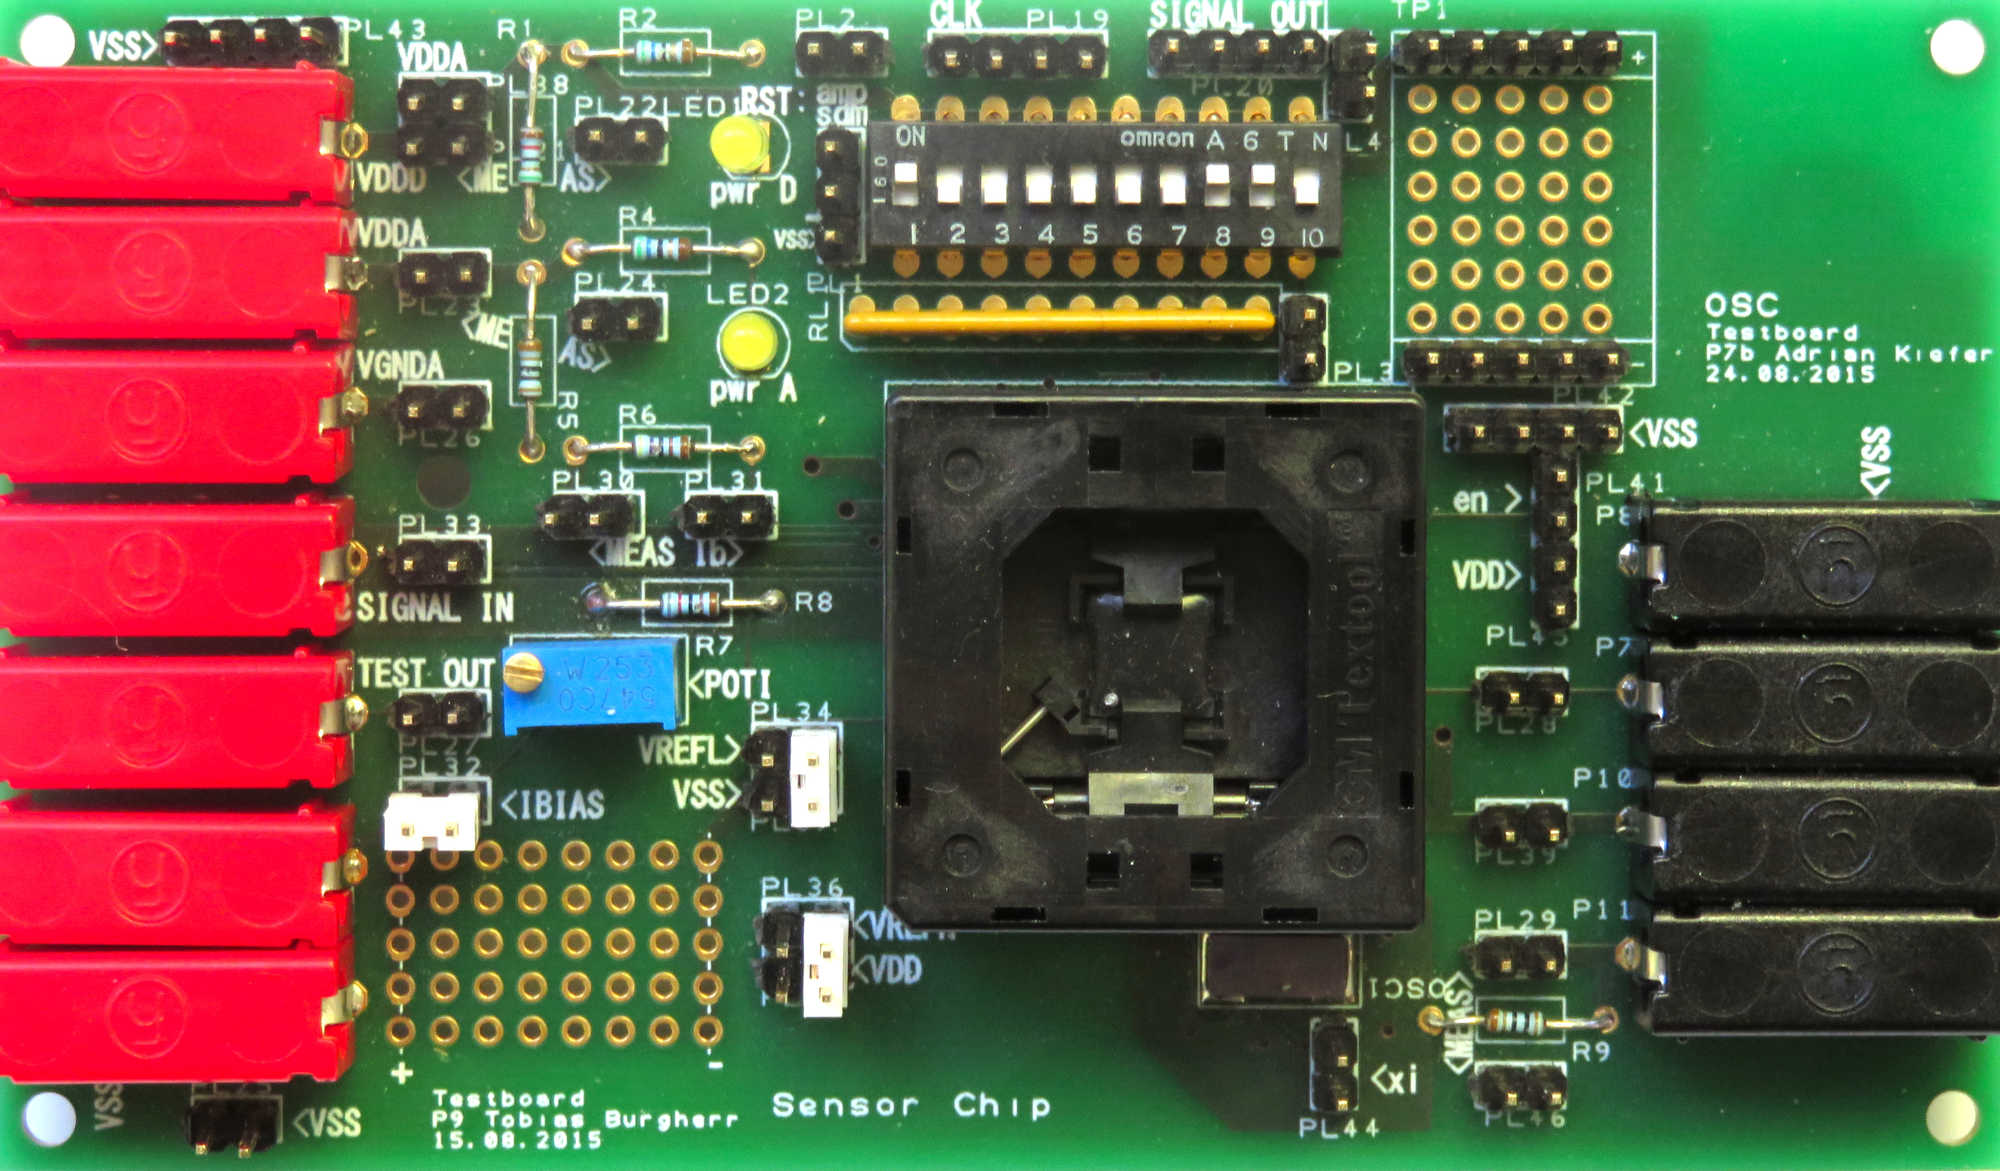
\includegraphics[width=135mm]{images/pcb/pcbOverview.jpeg}};
    \end{scope}
    %\node[fill=black,text=white,anchor=south west] at (0mm,0mm) {\textsf{\Large{VDDD}}};

    \node[%
        %fill=black,
        %fill opacity=0.5,
        text=white,
        text opacity=1,
        rounded corners=1mm,
        anchor=south west] at (4mm,66mm) {\plugtext{VDDD}};

    \node[%
        %fill=black,
        %fill opacity=0.5,
        text=white,
        text opacity=1,
        rounded corners=1mm,
        anchor=south west] at (4mm,56.5mm) {\plugtext{VDDA}};

    \node[%
        %fill=black,
        %fill opacity=0.5,
        text=white,
        text opacity=1,
        rounded corners=1mm,
        anchor=south west] at (4mm,47.5mm) {\plugtext{VGNDA}};

    \node[%
        %fill=black,
        %fill opacity=0.5,
        text=white,
        text opacity=1,
        rounded corners=1mm,
        anchor=south west] at (1mm,37.5mm) {\textbf{\textsf{\large{SIGNAL IN}}}};

    \node[%
        %fill=black,
        %fill opacity=0.5,
        text=white,
        text opacity=1,
        rounded corners=1mm,
        anchor=south west] at (1mm,27.5mm) {\textbf{\textsf{\large{TEST OUT}}}};

    \node[%
        %fill=black,
        %fill opacity=0.5,
        text=white,
        text opacity=1,
        rounded corners=1mm,
        anchor=south west] at (4mm,17mm) {\plugtext{IBIAS}};

    \node[%
        %fill=black,
        %fill opacity=0.5,
        text=white,
        text opacity=1,
        rounded corners=1mm,
        anchor=south west] at (4mm,8mm) {\plugtext{VSS}};
\end{tikzpicture}

    \caption{Test board overview}
    \label{fig:pcbOverview}
\end{figure}

\begin{table}
    \centering
    \caption{Sensor chip toplevel pins}
    \label{tab:inputPlugs}
    \scriptsize
    \sisetup{list-pair-separator = { or }}
    \rowcolors{2}{solarized-base3}{white}
    \begin{tabular}{>{\fontfamily{jkptt}\selectfont}l>{\fontfamily{jkptt}\selectfont}lp{30mm}lp{30mm}} \\
    %\begin{tabular}{>{\fontfamily{lmtt}\selectfont}l>{\fontfamily{lmtt}\selectfont}lp{30mm}lp{30mm}} \\
        \toprule
        \textnormal{\textsc{Pin \#}} & \textnormal{\textsc{Name}}                  & \textsc{Description} & \textsc{Value} & \textsc{Note} \\
        \midrule
        39 & vin                     & analog input signal                         & \SIrange{0.5}{2.5}{\volt} & \\
        25 & bit\_stream             & digital output signal                       & \SIlist{0;3}{\volt}       & \\
        34 & clk                     & clock                                       & \SIlist{0;3}{\volt}       & \\
        36 & sdm\_rst                & pulse to reset the $\Sigma\Delta M$         & \SIlist{0;3}{\volt}       & short pulse is enough (min $T_C$) \\
        41 & vgnda                   & analog ground                               & \SI{1.5}{\volt}           & \\
        48 & vrefh                   & high reference voltage                      & \SI{3}{\volt}             & \\
        47 & vrefl                   & low reference voltage                       & \SI{0}{\volt}             & \\
        46 & ibias                   & bias current                                & \SI{120}{\micro\ampere}   & $24 \cdot 5 \cdot 1$, internally reduced by 120 \\
        43 & sc\_amp\_vout\_test\_en & enables test output after preamp            & \SIlist{0;3}{\volt}       & \SI{0}{\volt}: off, \SI{3}{\volt}: on\\
        44 & sc\_amp\_vout\_test     & test output after preamp                    & \SIrange{0.5}{2.5}{\volt} \\
        33 & sc\_amp\_rst\_ext\_en   & enables external reset input for the preamp & \SIlist{0;3}{\volt}       & \SI{0}{\volt}: off, \SI{3}{\volt}: on\\
        32 & sc\_amp\_rst\_ext       & external reset input for the preamp         & \SIlist{0;3}{\volt}       & Internally synced to \signal{clk}. Needs \signal{en} signal. \\
        35 & sc\_amp\_pos\_neg\_amp  & positive or negative gain                   & \SIlist{0;3}{\volt}       & \SI{0}{\volt}: positive, \SI{3}{\volt}: negative \\
        28 - 31 & sc\_amp\_csel<3:0> & set gain                                    & \SIlist{0;3}{\volt}       & See table TODO \\
        27 & sc\_amp\_en             & enable preamp                               & \SIlist{0;3}{\volt}       & \SI{0}{\volt}: off, \SI{3}{\volt}: on\\
        26 & sah\_sdm\_en            & enable $\Sigma\Delta M$ S/H bock            & \SIlist{0;3}{\volt}       & \SI{0}{\volt}: off, \SI{3}{\volt}: on\\
        42 & vdda                    & analog positive power supply                & \SI{3}{\volt}             & \\
        37 & vddd                    & digital positive power supply               & \SI{3}{\volt}             & \\
        40 & vss                     & analog and digital negative power supply    & \SI{0}{\volt}             & \\
        \bottomrule
    \end{tabular}
    \sisetup{list-pair-separator = { and }}
\end{table}
\todo[inline]{insert table with gain list and reference in table 2.1}
\missingfigure{Overview of PCB, sections referenced}
\missingfigure{PCB Schematic}
\missingfigure{Chip Socket}




% ---------------------------------------------------------------------------- %
\subsection{Supply Voltages, Input Signal and PCB Settings}
\label{subsec:supplyVoltagesAndSettings}
% ---------------------------------------------------------------------------- %

\todo[inline]{bias current resistors}
\todo[inline]{supply voltages, Power Supplies}
\todo[inline]{DIP Switches}
\todo[inline]{Clock: between 0V and 3V, not -1.5 and +1.5}
\todo[inline]{Output impedance of signal generators}
\todo[inline]{Jumpers for some sockets}
\missingfigure{Bias Current Resistors}
\missingfigure{Power Supplies}
\missingfigure{Signal Generators}
\missingfigure{Cabling}
\missingfigure{Multimeters}
\missingfigure{Oscilloscope}


% ---------------------------------------------------------------------------- %
\subsection{Setting up the Raspberry Pi}
\label{subsec:setupRaspbi}
% ---------------------------------------------------------------------------- %

\todo[inline]{installation}
\todo[inline]{voltages, connections w/ test board}


% ---------------------------------------------------------------------------- %
\subsection{Performing Measurements}
\label{subsec:performingMeasurements}
% ---------------------------------------------------------------------------- %

\todo[inline]{Reading Data on Raspbi}
